\newpage
\section{Ergebnisse}
\label{sec:ergebnisse}
%Was waren die Ergebnisse der Untersuchungen?

In diesen Abschnitt werden die Ergebnisse zur Verdickungsmitteldosierung dargestellt. Nach Verifizierung des Problems und dessen Beschreibung erfolgen die Ergebnisse der Untersuchungsmethoden, sowie Entscheidungsverfahren für die Verfahrensplanung und schlussendlich die technische Umsetzung einer Dosiervariante mit einer Gefährdungsbeurteilung.

\subsection{Verifizierung und Analyse des Dosierproblems}
Im ersten Schritt wurde der Ist-Zustand der Dosierung erfasst, sowie die Gegebenheiten im Werk analysiert. Danach erfolgte das Zusammentragen der Anforderungen an eine halbautomatisch umgesetzte Dosierung.
 
\subsubsection{Ist-Zustand: Produktionsweise und aktuelles Dosierverfahren}
Das herzustellende Produkt für das eine halbautomatische Verdickerdosierung umgesetzt werden soll nennt sich \textit{AC 548}. Es ist eine Acrylat-Copolymer Dispersion und kann für Bautenfarben, Lacke, wärmeaktivierbare Klebstoffe und Putze verwendet werden. Internen Aussagen zufolge wird es hauptsächlich für Buntsteinputze genutzt. \todo{Quellenangabe} Produziert wird \textit{AC 548}, wie alle Produkte der \textsc{Alberdingk Boley Leuna GmbH}, im Batch-Betrieb à \SI{14}{\tonne} und wird vorzugsweise in Kampagnen geplant.\linebreak
Derzeit wird für dieses Produkt das Verdickungsmittel Rheobyk-H 3300 VF der \textsc{Byk-Chemie GmbH} eingesetzt, welches jedoch im Laufe des Jahres 2022 durch Einstellen der Produktion mit dem Verdickungsmittel TAFIGEL PUR 85 der \textsc{Münzing Chemie GmbH} substituiert werden soll. Die aktuelle Dosierung beläuft sich dabei auf die Nutzung eines \SI{0}{\liter}-Kunststofffasses als Dosierbehälter. Hierfür werden zunächst \SI{22}{\kilo \gram} des Verdickungsmittels in einem "`Transportfass"' im Chemikalienlager abgewogen und dann am entsprechenden Einstelltank bereit gestellt. Für den Start der Dosierung wird das "`Dosierfass"', welches mit einem Dosierloch an der Fassunterseite versehen ist, in das Fallschutzgitter des Mannlochs gehängt und der Inhalt des Transportfasses in das Dosierfass gekippt. Dargestellt ist diese Art der Dosierung in Abbildung \ref{fig:aktuelle_dosierung}.

\begin{figure}[h!]
	\centering
	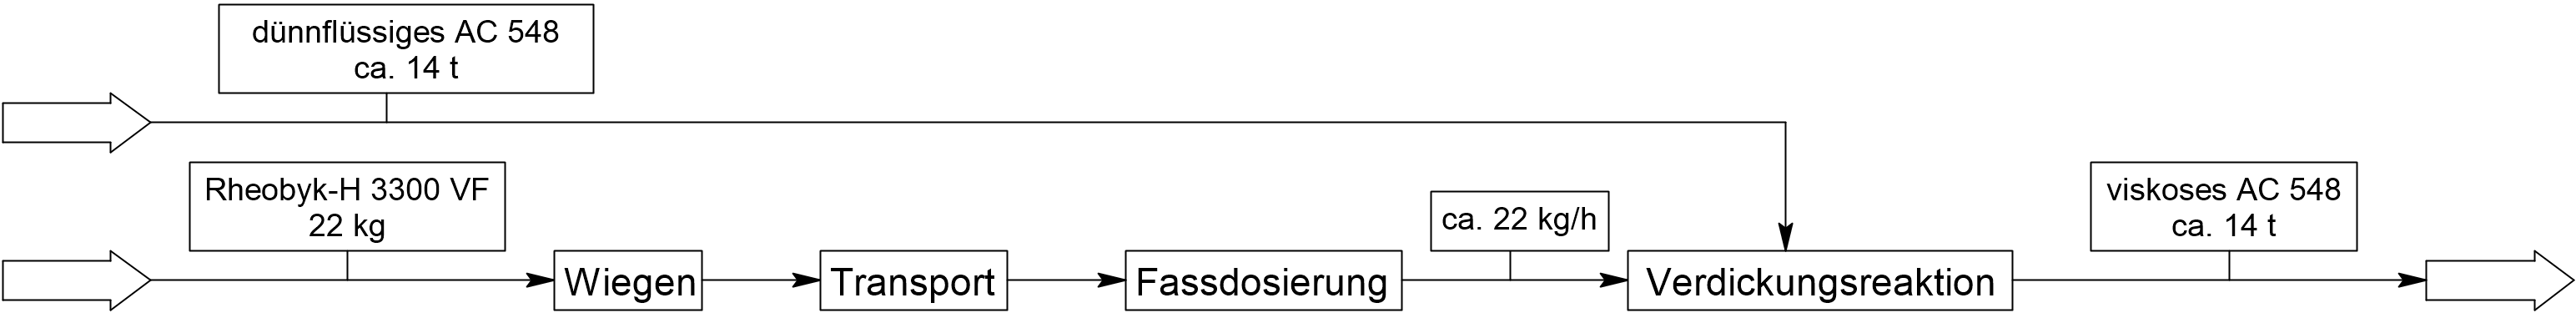
\includegraphics[width=\textwidth]{img/aktuelle_dosierung}
	\caption{Aktuelle Dosierung des Verdickungsmittels Rheobyk-H 3300 VF}
	\label{fig:aktuelle_dosierung}
\end{figure}
\FloatBarrier
%Ende

Vorteile dieses Dosierverfahrens sind die einfache und kostengünstige Umsetzung. Nachteilig ist jedoch, dass man neben dem "`Dosierloch"' und dem Fass selbst keine Einstellparameter vorhanden sind und der Dosierstrom weder messtechnisch erfasst noch im Prozessleitsystem (PLS) einsehbar ist. Zudem kann die Umsetzung für die Dosierung nur bedingt hygienisch erfolgen.

\subsubsection{Soll-Zustand: Anforderung an die Dosierung}
Die Anforderungen an eine automatisierte Dosierung gliedern sich in mehrere Interessensgruppen auf. Beginnend mit der \textit{Technik}, sollen unter diesem Begriff jegliche Anforderungen der Prozess- und Sicherheitstechnik beschrieben sein. Beispielsweise fallen darunter die Dosierrate, die Dosiergenauigkeit, Ex-Schutz der beachtet werden muss und Weiteres. Die zweite Gruppierung beschreibt die Anforderungen der \textit{Produktion}, sprich die Interessen der auszuführenden Chemiefacharbeiter in der Anlage. Eine Forderung stellt dabei die einfache Bedienbarkeit dar. Zuletzt soll jedoch auch die \textit{Wartung} entsprechend leichtgängig und der Verschleiß des Dosiersystems gering sein. Alle Forderungen der verschiedenen Perspektiven sind in Tabelle \ref{tab:anforderungen} zusammenfasst und wurden durch erfragen des Personals und durch vorgegebenen Prozessparametern ermittelt.

% Table generated by Excel2LaTeX from sheet 'Daten'
\begin{table}[h!]
	\renewcommand*{\arraystretch}{1.2}
	\centering
	\caption{Anforderungen an die Verdickungsmittel-Dosierung}
	\label{tab:anforderungen}
	\resizebox{\textwidth}{!}{
		\begin{tabulary}{1.2\textwidth}{LL|L|L}
			\hline
			\multicolumn{2}{l|}{\textbf{Technik}} & \textbf{Produktion} & \textbf{Wartung}\\
			\hline
			Dosierrate: & 22 bis \SI{44}{\kilo \gram \per \hour}&einfache Bedienbarkeit&geringer Verschleiß\\
			Dosiergenauigkeit: & $\pm \, \SI{200}{\gram}$	& leichte Reinigung & leichte Wartung\\
			Ex-Schutz:	 & Zone 2 &Zeitersparnis&\\
			Risiko:  &minimal&&\\
			Verdickungsmittel: &TAFIGEL PUR 85&&\\
			Prozessleitsystem: &im PLS einsehbar&&\\
			Adaptierbarkeit:& für weitere Tanks adaptierbar &&\\
			Aufstellungsort: &siehe Abbildung \ref{fig:aufstellungsort}&&\\
			\hline
	\end{tabulary}}
\end{table}%
\FloatBarrier

Da weder die geforderte Dosiergenauigkeit erfasst noch der Dosierstrom in der aktuellen Dosierung gemessen wird, ist der Unterschied zwischen Ist- und Soll-Anforderung an die Dosierung bereits erfüllt und das Problem somit als solches verifiziert. Außerdem setzt die derzeitige Dosierung eine gewisse Fließfähigkeit durch das Verdickungsmittel Rheobyk-H 3300 VF voraus, welche das TAFIGEL PUR 85 möglicherweise nicht erfüllt.

\begin{figure}[h!]
	\begin{minipage}[b]{0.475\textwidth}
		\centering
		\includegraphics[height=4.25cm]{img/aufstellungsort}
		\caption{Aufstellungsort für Dosierung}
		\label{fig:aufstellungsort}
	\end{minipage}
	%\hspace*{0.05\textwidth}
	\begin{minipage}[b]{0.475\textwidth}
		\centering
		\includegraphics[height=4.25cm]{img/flansch}
		\caption{Flansch für Dosierstrom}
		\label{fig:flansch}
	\end{minipage}
\end{figure}
\FloatBarrier

%geringer Verschleiß
%leichte Wartung
%einfach zu Bedienen
%leichte Reinigung --> Spülbarkeit
%Dosiergenauigkeit und DOsierstrom
%--> SAmmeln von Informationen im Werk
% Platz im Werk mit Geometrie
%
%Kampagne
%Mitarbeiterkosten sparen
%Zeitersparnis
%Einfachheit
%Ex-Schutz
%PLS
%Prozesssicherheit

\subsubsection{Eigenschaften des Verdickungsmittels}
In der geplanten Dosierung soll auf das Verdickungsmittel TAFIGEL PUR 85 der \mbox{\textsc{Münzing Chemie Gmbh}} zurückgegriffen werden. Laut Hersteller handelt es sich hierbei um einen assoziativen Polyurethan-Verdicker, welcher durch Gerüstbildung zwischen Verdickermolekülen, Bindemittel und Pigmentpartikeln die gewünschte Viskosität hervorruft und stabilisiert. Diese Beschreibung deckt sich mit den vorangegangenen Beschreibung der Assoziativverdicker.\cite{MunzingChemieGmbH.2014}\\
--> Datenblätter

\subsubsection{Viskositätsmessungen}
--> nach DIN
--> beide Verdickungsmittel

\subsubsection{Verdünnungsverhalten}
--> Eigenregie

\subsubsection{Erwärmungsverhalten}

--> beim Hersteller angefragt

\subsubsection{Pumpversuche}

erster Volumenstrom erst nach einer Stunde zu erkennen 


\todo[inline]{Entscheidungsprobleme werden aufgrund des Umfangs und der schweren Nachvollziehbarkeit nicht dargestellt}

\subsection{Problem: Entscheidung für ein Verfahren}
%Verdünnen
%spülen
%erwrämen
%nichts 
%Rühren
%kombinationen
%aktuelles Verfahren

\subsection{Problem: Entscheidung für Gebindetyp}
%Preis nachfrage
%\subsubsection{Angebotsanfrage}
%\subsubsection{Entscheidungsverfahren}

\subsection{Problem: Direkte Zugabe mit Pumpe oder Dosierbehälter}

\subsection{Problem: Auswahl des Pumpentyps}
%\subsubsection{Literaturarbeit}
%Bücher gelesen für Auswahlhilfe
%\subsubsection{Fachgespräche und Angebotsanfrage}
%\subsubsection{Entscheidungsverfahren}

%\subsection{Auswahl des Pumpentyps, sowie des Leitungsdurchmessers}
%Gespräche geführt und Leitung hat sich nach möglichen Drücken in der Anlage und Pumpentyp, sowie Berechnungen gerichtet gerichtet

\subsection{Problem: Messverfahren}

\subsection{Technische Planung für Verdickungsmitteldosierung}
\subsubsection{Verfahrensfließbild der Verdickerdosierung}
\subsubsection{R\&I- Fließbild der Verdickerdosierung}
\subsubsection{Theoretische Rohrleitungsplanung der Verdickerdosierung}
%vertretbarer Druckverlust
%Rohrdurchmesser und Nenndruck
%--> Rohrleitungsklassifizierung

\subsubsection{Signalverarbeitungsplanung der Verdickerdosierung}

\subsection{Gefährdungsbeurteilung der geplanten Verdickungsmitteldosierung}


